\hypertarget{ch2}{\chapter{Theoretical description of selected statistical models}}

This chapter introduces a theoretical description of the two statistical models that were used in this thesis. They exploit fundamentally different principles based on which the process is modeled. We will describe the \textit{Facebook Prophet} model (interchangeably called \textit{the Prophet}), which is used for changepoints detection. Then the \textit{Seasonal Autoregressive Integrated Moving Average} (SARIMA) model will be covered. 

To argue our choice from the real-world applications point of view, it is necessary to introduce other studies that aim at the same problem. 

In Sengupta et al. \cite{Sengupta2020.06.25.20140004} different machine learning models such as various types of regression, LSTM (Long short-term memory) deep learning forecasting model, ARIMA, and the Facebook Prophet were compered during modeling of the COVID-19 time series related to India. Results reported by the authors of this study suggest that the ARIMA and Prophet models achieved more significant prediction results (on average) than most alternatives.

In Wang et al. \cite{WANG2020110058} authors used the Facebook Prophet logistic model for predicting the epidemic trend of COVID-19 in the whole world, Brazil, Russia, India, Peru, and Indonesia.

In Indhuja et al. \cite{indhuja2020prediction}, the Facebook Prophet model was used for modeling the explosive growth number of new cases in India.

In ArunKumar et al. \cite{ARUNKUMAR2021107161} were achieved quite good results in forecasting the dynamics of COVID-19 cases (confirmed, active, and death) for 16 countries around the world using the SARIMA model. 

In Ceylan et al. \cite{CEYLAN2020138817} the bunch of ARIMA models was used for forecasting the COVID-19 pandemic processes in Spain, Italy, and France. This study also refers to various researches made in the past that use (S)ARIMA models during the modeling of different diseases such as Malaria, Severe Acute Respiratory Syndrome, and so on.

Now we can move to the detailed description of the selected models.

\section{Facebook Prophet model}

The Facebook Prophet model was presented to the public and released in open source in 2017. The main objectives set forth by the creators are to simplify the modeling of processes whose evolution changes over time and to create a model that will be easily tuned during working on real-world projects.

This section mainly follows the explanation that can be found in the "Forecasting at Scale" article that introduces the Prophet model \cite{Taylor2018}.

\subsection{Main equation}

In essence, the Prophet uses a decomposable additive time series model with three basic components: trend, seasonal, and holidays. More formally:

\begin{definition}[\textbf{Prophet model main equation}]
\textit{Let us assume a time series $Y = \left\{Y_{t}\;|\;t \in T\right\}$ where  $Y_{t}$ is the value of observed variable $Y$ at timestamp $t$. The basic equation behind the Prophet model is
\begin{equation}
    Y_t = g(t) + s(t) + h(t) + e(t),
\label{eq_Prophet}
\end{equation}
where the variables are as follows:
\begin{itemize}
    \item $Y_{t}$ --- value of the observed variable in timestamp $t$.
    \item $g(t)$ --- trend component (non-periodic changes over time).
    \item $s(t)$ --- seasonal component (describes periodic changes over time).
    \item $h(t)$ --- holidays component (effect of irregular schedules $\geq$ 1 day long).
    \item $e(t)$ --- changes not covered by the model (error term).
\end{itemize}}
\end{definition}

Now, let us focus on each component separately.

\subsection{Trend component models} 
Prophet model has two options for trend modeling:
\begin{itemize}
    \item \textbf{Piecewise linear model}
    \item \textbf{Saturation growth model}
\end{itemize}

\subsubsection{Linear growth model}

We can use a linear model for processes where the maximum or minimum value of the observed variable is not defined, and we do not need saturation near it. However, it is well known that simple linear models cannot describe the process with lots of slope changes. 

For situations like this,  we must introduce a linear piecewise model. This model assumes the constant growth rate with changepoints. It is the standard model and used to be the default option in Prophet. 

To introduce the piecewise model equation, we need to formulate the definition of the vector of rate adjustments.
\begin{definition}[\textbf{Vector of rate adjustments}]
\textit{Let us assume that we have a time series with observed value $y$ which depends on time and has $C$ changepoints at timestamps $c_j$, $j$ = $1$, \ldots, $C$. That can be described as a vector of rate adjustments
\begin{equation}
    \boldsymbol{\delta} \in R^C,
\label{eq_adj_vector}
\end{equation}
where $\delta_{j}$ is a change in rate of trend growth at timestamp $c_j$.}
\end{definition}

According to this definition, the growth rate at any timestamp $t$ can be described as
\begin{equation}
    b + \sum_{j} \delta_{j}, \quad \text{while} \; t > c_j,
\end{equation}
\textit{where b $is$ a base growth rate at timestamp $t_{0}$.}
This rate change can be represented like a vector $a(t)$ in $\left\{0, 1\right\}^{C}$ such that: 
\begin{equation}
    a_{j}(t)=   \left\{
\begin{array}{ll}
      1, & \text{if} \; t \geq c_j, \\
      0, & \text{if} \;t < c_j. \\
\end{array} 
\right.  
\label{eq_used_changepoint_vector}
\end{equation}
The rate at timestamp $t$ then is 
\begin{equation}
b + \mathbf{a}(t)^{T}\boldsymbol{\delta}.
\label{eq_growth_rate_t}
\end{equation}

\begin{figure}[!ht]
\centering
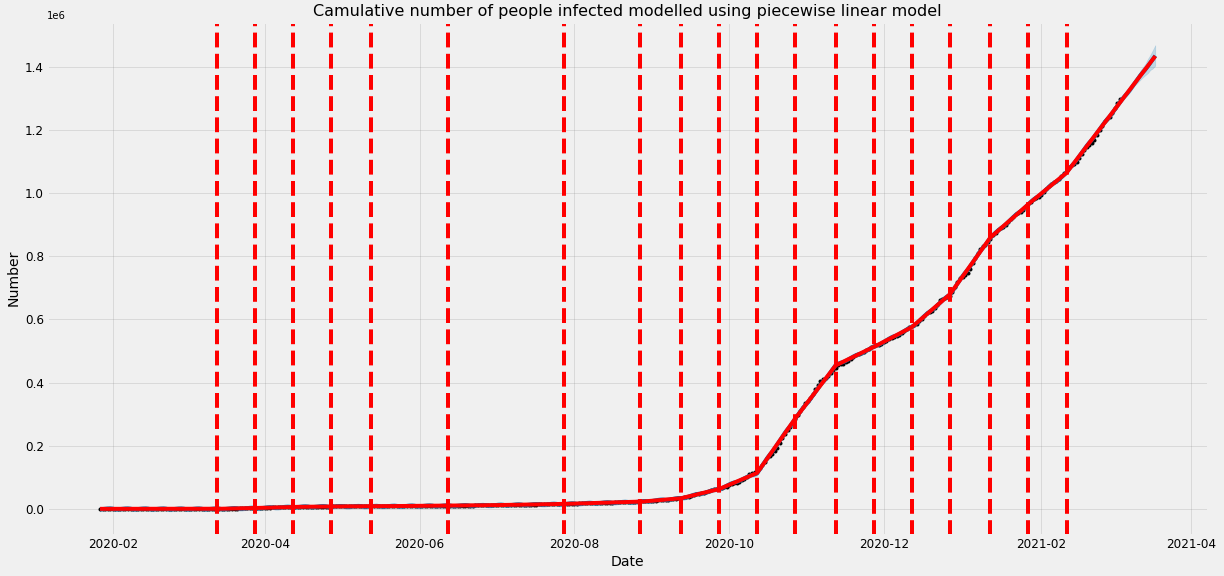
\includegraphics[width=1\textwidth, height=0.5\textwidth]{figures/chapter_03/picewise_model_example.png}
\caption{The cumulative number of people infected in Czech Republic time series modeled using the Facebook Prophet piecewise linear model with normally distributed changepoints for the first 90\% of the time series.}
\label{fig:piecewise_example}
\end{figure}

In addition to the base growth rate $b$, it is possible to tune the offset parameter $m$ (the value of the midpoint, where the slope changes its direction). This parameter is used to make the function continuous and connect the endpoints of the segments between changepoints:
\begin{equation}
    m + \mathbf{a}(t)^{T}\boldsymbol{\gamma},
\end{equation}
\textit{where components of the vector $\boldsymbol{\gamma}$ are defined as $\gamma_j = -c_{j}\delta_{j}$.}

After specifying all these parts, we can formulate the final equation of the piecewise linear model.

\begin{definition}[\textbf{Peicewice linear model}]
\textit{Let $g(t)$ be the value of trend component $g$ at timestamp $t$. Then the piecewise linear model equation can be defined as (we use extra parentheses for better visibility)}
\begin{equation}
   g(t) = (b + \mathbf{a}(t)^{T}\boldsymbol{\delta})t + (m + \mathbf{a}(t)^{T}\boldsymbol{\gamma}),
   \label{eq_piecewise_linear_model}
\end{equation}
\textit{where the variables of the equation are:
\begin{itemize}
    \item $b$ --- base trend growth rate.
    \item $\mathbf{a}(t)$ --- vector that specifies changepoints used for calculation of growth rate at timestamp $t$.
    \item $\boldsymbol{\delta}$ --- vector of rate adjustments.
    \item $m$ --- offset parameter.
    \item $\boldsymbol{\gamma}$ --- vector of offset adjustments.
\end{itemize}}
\end{definition}

According to this equation, we compute the value of the trend component $g$ at timestamp $t$ by multiplying the amount of time passed from the beginning of a process and the growth rate at this timestamp $t$. After this, we add an offset parameter $m$ corrected using the vector of offset adjustments $\boldsymbol{\gamma}$ to make this function continuous.
In this thesis, the piecewise linear model will be primary, because it correctly fits almost all selected COVID-19 time series.

Figure \ref{fig:piecewise_example} introduces the example of the Facebook Prophet piecewise linear model with normally distributed changepoints for the first 90\% of the time series. The vertical dashed lines pass through the timestamps where the changepoints are located. 

\subsubsection{Nonlinear Saturation growth model}
Sometimes, there is a time series forecasting task where it is necessary to deal with the maximum or minimum possible value. For example, at the beginning of an epidemic process, the government cannot deal with a fast increase in the number of people infected. In this case we can see explosive (non-linear), or even nearly exponential growth. In situations like this, we can use the logistic growth model, which can be written as 
\begin{equation}
    g(t) = \frac{C}{1 + e^{-k(t - m)}},
    \label{eq_saturating_model}
\end{equation}
\textit{where $C$ is the carrying capacity, $k$ is the growth rate, and $m$ --- an offset parameter.}
To deal with more complex situations, there are some improvements 

\begin{figure}[!ht]
\centering
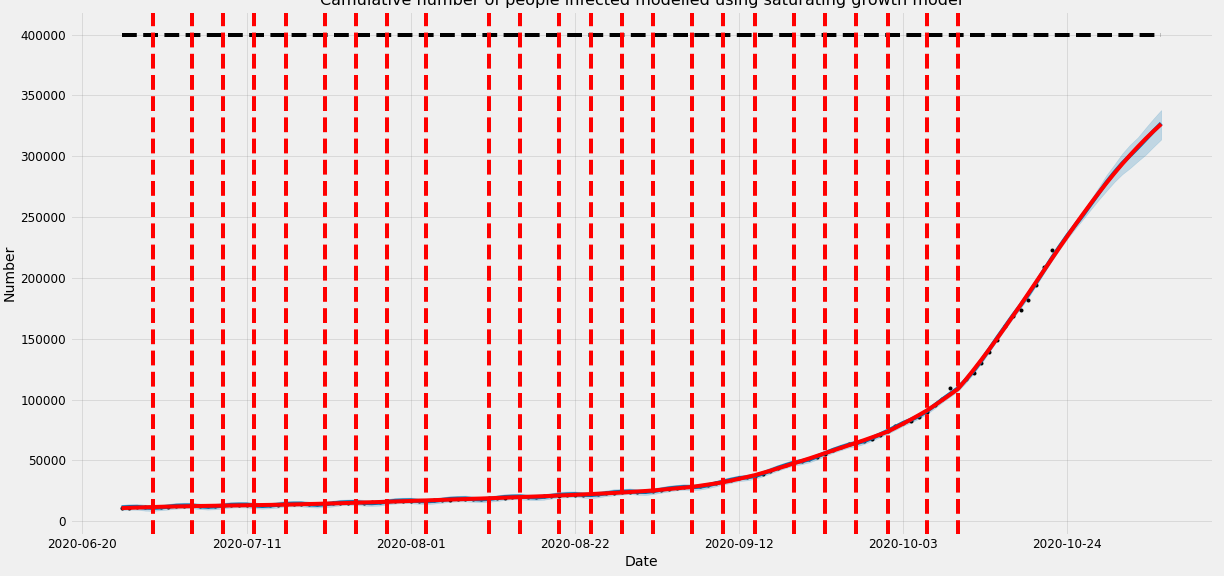
\includegraphics[width=1\textwidth, height=0.5\textwidth]{figures/chapter_03/logistic_model_example.png}
\caption{The cumulative number of people infected in Czech Republic time series (period of the explosive growth) modeled using the Facebook Prophet saturating growth model with normally distributed changepoints for the first 90\% of the time series.}
\label{fig:logistic_example}
\end{figure}

in the nonlinear version of the Prophet model. First, the constant carrying capacity $C$ was replaced with time-varying $C(t)$ (better for dynamic environments, where the maximum or minimum value changes over time). Second, the growth rate is changing (the same principle as in the linear model equation \ref{eq_growth_rate_t}). However, there is a difference associated with the offset parameter $m$. Its correct adjustment can be written as 
\begin{equation}
    \gamma_j = \bigg(c_j - m - \sum_{l < j} \gamma_l\bigg)\bigg(1 - \frac{b + \sum_{l < j} \delta_l}{b + \sum_{l \leq j} \delta_l}\bigg).
\end{equation}  
After all these corrections, we can formulate the final linear growth model equation.
\begin{definition}[\textbf{Logistic non-linear model}]
\textit{Let $g(t)$ be the value of trend component $g$ at timestamp $t$. Then the logistic (non-linear) model equation can be defined as
\begin{equation}
    g(t) = \frac{C(t)}{1 + exp(-(k + \mathbf{a}(t)^{T}\boldsymbol{\delta})(t - (m + \mathbf{a}(t)^{T}\boldsymbol{\gamma})))},
    \label{eq_logisic_model}
\end{equation}
where the variables are as follows 
\begin{itemize}
    \item $C(t)$ --- time-varying growth rate.
    \item $b$ --- base trend growth rate.
    \item $\mathbf{a}(t)$ --- vector that specifies changepoints used for calculation of growth rate at timestamp $t$.
    \item $\boldsymbol{\delta}$ --- vector of rate adjustments.
    \item $m$ --- offset parameter.
    \item $\boldsymbol{\gamma}$ --- vector of offset adjustments.
\end{itemize}}
\end{definition}

Figure \ref{fig:logistic_example} shows the part (with exponential growth) of the time series that describes cumulative number of people infected in the Czech Republic using the Facebook Prophet saturating growth model with normally distributed changepoints for the first 90\% of the time series. The capacity in the example is constant ($C(t) = 4000000$ for all $t$). 

\subsubsection{Automatic changepoints selection}
\label{sec:automatic_cp_detection}
The Prophet model supports manual changepoint selection. However, sometimes it is not available. In cases like this, for usage convenience, there is an automatic changepoint selection mechanism. It exploits a sparse prior on $\delta$ with equation \ref{eq_piecewise_linear_model} and \ref{eq_logisic_model}. In practice, we might specify a large number of changepoints (e.g., one or two per month) and use the prior $\delta_j \sim Laplace(0, \tau)$. 
\begin{definition}[\textbf{Classical Symmetric Laplace distribution }\cite{Kotz2001}]
\textit{We can say that a random variable has the Classical Laplace distribution on $(-\infty ; \infty)$ if its distribution is given by the density function 
\begin{equation}
    f(x, \theta, \tau) = \frac{1}{2\tau}exp\bigg(\frac{-|x - \theta|}{\tau}\bigg),
\end{equation} 
where $\theta \in (-\infty ; \infty)$ is the location parameter and $\tau > 0$ is the scale parameter.} 
\end{definition}
The parameter $\tau$ controls the flexibility of the rate change. It has no effect on the base growth rate, so if $\tau$ goes to 0, we receive standard linear or logistic growth.

According to the official Facebook Prophet documentation \cite{ProphetDoc}, it specifies 25 potential normally distributed changepoints for the first 80\% of the time series (by default). Subsequently, some of them are discarded by a procedure exploiting a sparse prior distribution. While fitting the trend component\footnote{\url{https://github.com/facebook/prophet/issues/933} --- explanation from a Facebook Prophet contributor on the official GitHub page}, the Prophet model minimalizes the sum of components of the vector of rate adjustments $\delta$. In other words, it tries to specify a set of changepoints $C$ with the biggest possible number of $\delta_j = 0$.

\subsubsection{Trend forecast uncertainty}

With just only historical data, the forecasted trend will have a constant growth rate. We need to extend the generative model forward to estimate the forecast uncertainty. In the Prophet model, we have $C$ changepoints over a history of $T$ time points, each of which has a rate change $\delta_j \sim Laplace(0, \tau)$. We can simulate future rate changes by replacing $\tau$ with the variance obtained from historical data. To perform this, we can use a maximum likelihood estimate of the rate scale parameter: \begin{equation}
    \lambda = \sum_{j=1}^{C} \delta_j.
\end{equation} We need to save historical changepoint frequency, so future changepoints  are randomly selected according to the following principle: \begin{equation}
    \forall j > T,   \left\{
\begin{array}{ll}
      \delta_j = 0, & \text{with probability } \frac{T- S}{T}, \\
      \delta_j \sim Laplace(0, \lambda), & \text{with probability } \frac{S}{T}. \\
\end{array} 
\right.
\end{equation} This means an assumption that in the future we will have the same frequency and magnitude of rate changes. After receiving lambda from historical data, we use a generative model to estimate possible trends and calculate uncertainty intervals. However, this assumption is quite strong, and these intervals may have not exact coverage. 

Moreover, as we already said, parameter $\tau$ controls rate change flexibility in historical data, so by increasing it, we can achieve lower training error but wider uncertainty intervals.

\subsection{Seasonal component}
A large number of time series can have multiperiod seasonality (yearly, weekly, daily, or quarterly). To handle these effects, the Prophet model contains the seasonality model, which is represented by periodic functions of $t$. One of the best possible options for modeling time series periodic patterns is to use the Fourier series. 

Thus, let $P$ be a constant expected time series period (for example, $P = 7$ for weekly data with the daily time scale). We can use a \textit{standard trigonometric polynomial of order $N$} (in fact, it is the Fourier series \cite{tolstov1976fourier})
\begin{equation}
    s(t) = \sum_{n=1}^{N}\bigg(a_{n}\cos\frac{2\pi nt}{P} + b_{n}\sin\frac{2\pi nt}{P}\bigg),
    \label{eq_fourier_seires}
\end{equation}
which can approximate a wide range of seasonal patterns. There is no intercept in this equation because we already have the trend component. 

According to Equation \ref{eq_fourier_seires}, the seasonal component fitting requires $2N$ parameters, that can be represented as a vector $\beta = [a_1, b_1, \ldots, a_N, b_N]^T$. The Prophet model does this by constructing a matrix of seasonal vectors for each timestamp t in historical and future data. For example, for weekly seasonality and $N = 5$: \begin{equation}
    \mathbf{X}(t) = \bigg[\cos\bigg(\frac{2\pi \cdot 1 \cdot t}{7}\bigg), \ldots, \sin\bigg(\frac{2\pi \cdot 5 \cdot t}{7}\bigg)\bigg].
\end{equation} After defining all this, we can formulate a definition of the seasonal component of the Prophet model.

\begin{definition}[\textbf{Facebook Prophet Seasonal component}]
\textit{Let us assume the Facebook Prophet model main equation $Y_t = g(t) + s(t) + h(t) + e(t)$, which represents the decomposed value of the observed variable $Y$  at a timestamp $t$, then the seasonal component $s(t)$ can be defined as
\begin{equation}
    s(t) = X(t)\boldsymbol{\beta},
\end{equation}
where 
\begin{itemize}
    \item $\mathbf{X}(t)$ is a matrix of seasonal vectors for each timestamp $t$.
    \item $\boldsymbol{\beta} \sim \mathcal{N}(0, \sigma^2)$ is a vector of fitting parameters that applies a smoothing prior to the seasonality.
\end{itemize}}
\end{definition}

In practice, there are several possible values of $N$, and there arises the need to discriminate among them (for example, a bigger value can lead to overfitting but allows modeling of seasonal patterns that change faster). The \textit{Akaike information criterion} (AIC)  or the \textit{Bayesian information criterion} (BIC) are two popular criteria that (loosely speaking) quantify the model quality \cite{doi:10.1177/0049124104268644}.

\subsection{Holidays component}

This component is used to handle important irregular schedules that can effect forecasts.

For each holiday $i$, let assume $D_i$ as a set of past and future dates of this holiday. Then, to indicate that a timestamp $t$ takes place during holiday and to assign each holiday a parameter $k_i$ which will indicate a corresponding change in the forecast we need to specify the matrix of regressors $\mathbf{Z}(t)$: \begin{equation}
    Z_{i}(t)=   \left\{
\begin{array}{ll}
      1, & \text{if } t \in D_i, \\
      0, & \text{if } t \notin D_i. \\
\end{array} 
\right.
\end{equation}
Now we can define the holidays component more formally.
\begin{definition}[\textbf{Facebook Prophet Holidays component}]
\textit{Let us assume the Facebook Prophet model main equation $Y_t = g(t) + s(t) + h(t) + e(t)$, which represents the decomposed value of the observed variable $Y$  at a timestamp $t$, then the holidays component $h(t)$ can be defined as
\begin{equation}
h(t) = \mathbf{Z}(t) \cdot \mathbf{k}.
\end{equation} where 
\begin{itemize}
    \item $\mathbf{Z}(t)$ is a matrix of regressors.
    \item $\mathbf{k}$ is a vector of corresponding (to selected holidays) changes in the forecast.
\end{itemize}}
\end{definition}

In addition to the curtain holiday date, we can define a few-day window around it to handle extra weekends, and so on. Moreover, the Prophet model uses $\mathbf{k} \sim \mathcal{N}(0, \sigma^2)$ to inflict a smoothing prior on the holidays component.

\subsection{Model fitting}

Fitting the Facebook Prophet model means the estimation of different model parameters described in the previous subsections (smoothing prior, Fourier Series order, etc.). It is an optimization task, where we need to minimize the error between historical data and model \cite{ProphetDoc}.

\subsection{Forecast accuracy evaluation}

The Prophet model uses a time series compatible version of the cross-validation concept. It specifies the cutoff points in historical data and for each of them fits the model. Then it forecasts the following points (the amount is specified by the forecast horizon) and compares the forecasted and actual values. To measure accuracy for each forecast made during cross-validation, the Prophet can use, for example, \textit{Mean Absolute Percentage Error} (MAPE) defined as 
\begin{equation}
    MAPE = \frac{100}{n} \sum_{t=1}^{n}\Big|\frac{Y_t - \hat{Y_t}}{Y_t}\Big|,
\end{equation}
where $n$ is an amount of forecasted points, $Y_t$ is the real value of the observed variable $Y$ at timestamp $t$, and $\hat{Y_t}$ is the forecasted value at timestamp $t$. This formulation is similar to the definition in Hyndman et al. \cite{Hyndman2018} (Chapter 3.4, Evaluating forecast accuracy).

After calculation of the error for each forecast made during the cross-validation, the Prophet model computes the mean between all these errors.

\subsection{Summary}

The Facebook Prophet is an additive model that can be used in complex real-world tasks. It supports trend growth rate changes, multivariate seasonality, and irregular schedules. It uses complex methods for parameter estimation and forecast accuracy evaluation. 

In addition to this, we found out that the Prophet model is widely used for modeling the COVID-19 pandemic processes. 

All of the above properties led us to the fact that the Prophet model would be a good choice for statistical modeling of time series related to the COVID-19 pandemic.

\section{SARIMA model}

In this section, we will introduce the basic concepts behind common parametric models, created and used in practice to describe real-world processes. This category was named \textit{Autoregressive Moving Average Models} (ARMA).

However, it is important to describe \textit{Autoregressive} and \textit{Moving Average} processes and models separately.

\subsection{Autoregressive process, AR model}

In essence, autoregressive processes are regressions on themselves \cite{cryer2008time}. The autoregressive process of $p$th-order means that value at timestamp $t$ depends on values at $p$ the most recent timestamps before it. For future work, we will need a formal definition for this type of a process.

\begin{definition}[\textbf{Autoregressive process of order $p$} \cite{shumway2011}]
\textit{Let us assume a stochastic process $Y = \left\{Y_{t}\;|\;t \in T\right\}$. This process can be named \textbf{the autoregressive of order $p$} if it has the following form
\begin{equation}
    Y_t = \phi_{1}Y_{t-1} + \phi_{2}Y_{t-2} + \ldots + \phi_{p}Y_{t-p} + e_t,
    \label{eq_ar_process}
\end{equation}
where the elements of the equation are 
\begin{itemize}
    \item $\phi_1, \ldots, \phi_p$ --- autoregressive coefficients ($\phi_p \neq 0$).
    \item $Y_{t-1}, \ldots, Y_{t-p}$ --- most recent $p$ past values.
    \item $e_t \sim \mathcal{N}(0, \sigma^2)$ --- Gaussian white noise at timestamp $t$, unless otherwise stated. In fact, it is part of the $Y_t$ that can not be described using $Y_{t-1}, \ldots, Y_{t-p}$.
\end{itemize}
If we talk about the AR process with nonzero mean value $\mu$, we need to replace $Y_t$ with $Y_t - \mu$ in Equation \ref{eq_ar_process},
\begin{equation}
    Y_t - \mu = \phi_{1}(Y_{t-1} - \mu) + \phi_{2}(Y_{t-2} - \mu) + \ldots + \phi_{p}(Y_{t-p} - \mu)+ e_t,
\end{equation}
or write
\begin{equation}
    Y_t = \phi_{0} + \phi_{1}Y_{t-1} + \phi_{2}Y_{t-2} + \ldots + \phi_{p}Y_{t-p} + e_t,
    \label{eq_ar_process_non_zero_mean}
\end{equation}
where $\phi_0 = \mu(1 -  \phi_0 -  \phi_1 - \ldots - \phi_p)$.}
\end{definition}

For modeling this process, we can use the autoregressive model (abbreviated as \textbf{AR}($p$), where $p$ is an order of the autoregressive process). However, this model assumes that the process is \textit{stationary}. 

\subsubsection{Stationarity of AR process}

First, we need to define the backshift operator \cite{shumway2011}, which allows a more compact and readable mathematical form of some definitions and equations that will occur in the following subsections. 

\begin{definition}[\textbf{Backshift operator}]
\textit{Let $Y_t$ be a value of an observed variable $Y$ at timestamp $t$. Then the \textbf{backshift operator} $B$ is defined by
\begin{equation*}
    BY_t = Y_{t-1},
\end{equation*}
and extended to powers $B^{2}Y_{t} = B(BY_t) = BY_{t-1} = Y_{t-2}$, and so on. Therefore, \begin{equation}
    B^{k}Y_t = Y_{t-k}.
    \label{eq_backshift_operator}
\end{equation}}
\end{definition} 

Now we can rewrite the AR model from Equation \ref{eq_ar_process} using the backshift operator as
\begin{equation}
\begin{aligned}
    Y_t &= \phi_{1}Y_{t-1} + \phi_{2}Y_{t-2} + \ldots + \phi_{p}Y_{t-p} + e_t, \\
    e_t &= Y_t - \phi_{1}Y_{t-1} - \phi_{2}Y_{t-2} - \ldots - \phi_{p}Y_{t-p} \\
        &= Y_t - \phi_{1}BY_t - \phi_{2}B^{2}Y_t - \ldots - \phi_{p}B^{p}Y_{t-p} \\
        &= (1 - \phi_{1}B - \phi_{2}B^2 - \ldots - \phi_{p}B^p)Y_t \\
        &= \phi(B)Y_t,
    \label{eq_ar_operator}
\end{aligned}
\end{equation}
where $\phi(B)$ is an \textbf{autoregressive operator}. In essence, it is the \textbf{AR characteristic polynomial}, that will be introduced later in Definition \ref{def_ar_char_polynomial}.

This form of Equation \ref{eq_ar_process} is widespread and used in equations related to more complex models.

Now, for understanding the stationarity of an AR process, we might also define its characteristic polynomial \cite{cryer2008time}.

\begin{definition}[\textbf{AR process characteristic polynomial}]
\textit{Let us assume an AR process with zero mean ($\phi_{0} = 0$), $Y_t = \phi_{1}Y_{t-1} + \phi_{1}Y_{t-1} + \ldots + \phi_{p}Y_{t-p} + e_t$, then the \textbf{AR polynomial} is defined as \begin{equation}
    \phi(x) = 1 - \phi_{1}x - \phi_{2}x^2 - \ldots - \phi_{p}x^{p},
    \label{eq_ar_polynomial}
\end{equation} where $\phi_1, \ldots, \phi_p$ are the regression coefficients, and $x^1, \ldots, x^p$ are the complex numbers.
Therefore, the corresponding \textbf{AR characteristic equation} is \begin{equation}
    1 - \phi_{1}x^{1} - \ldots - \phi_{p}x^{p} = 0.
    \label{eq_ar_pol_eq}
\end{equation}}
\label{def_ar_char_polynomial}
\end{definition}
According to the definition of the white noise process, we assume that $e_t$ is independent from $Y_t, Y_{t-1}, \ldots, Y_{t-p}$. Thus, according to the stationarity condition of AR process (Box et al. \cite{box1976time}), we can now formulate the following definition.

\begin{definition}[\textbf{Stationarity condition of AR($p$) process}]
Let us assume the AR process of order $p$ with the characteristic polynomial $\phi(x)$ and the corresponding characteristic equation $\phi(x) = 0$. This process is \textbf{stationary}
\begin{itemize}
    \item{if the roots of characteristic equation $\phi(x) = 0$ all exceeded $1$ in absolute value, or in other words}
    \item{if both following conditions are satisfied:
        \begin{equation}
            \begin{rcases*}
            \phi_1 + \phi_2 + \ldots + \phi_p < 1 \\
            |\phi_p| < 1 \\
            \end{rcases*}
        \label{eq_stationarity_cond}
        \end{equation}}
\end{itemize}
\label{def_ar_stationarity}
\end{definition} 
\subsubsection{AR process autocorrelation function}

Assuming a stationary AR process with zero mean, we can now define an important recursive relationship \cite{cryer2008time} for the autocorrelation function as \begin{equation}
\begin{aligned}
    \rho_0 &= 1, \\ 
    \rho_{-k} &= \rho_{k}, \\
    \rho_k &= \phi_{1}\rho_{k - 1} + \phi_{2}\rho_{k - 2} + \ldots + \phi_{p}\rho_{k - p}, & \text{ for } k \geq 1.
\end{aligned}
\end{equation} This relationship is used to compute the numerical values of $\rho_k$ for all possible $k$.

\begin{figure}[!ht]
\centering
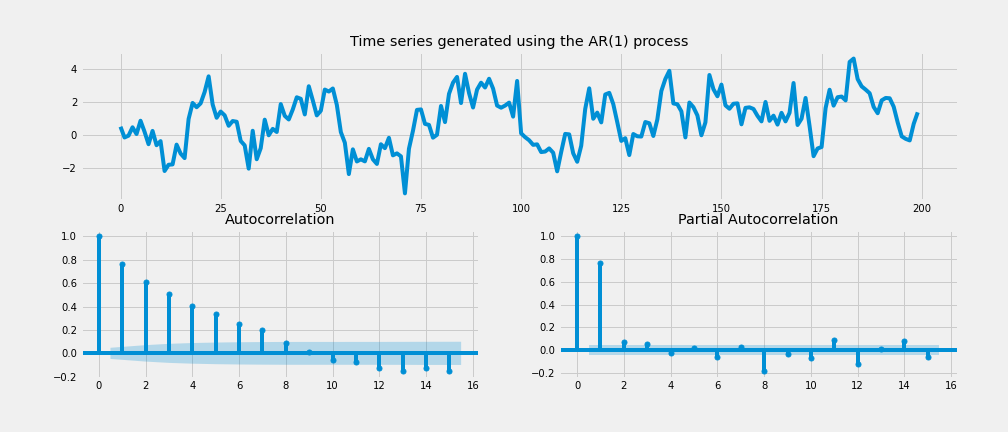
\includegraphics[width=1\textwidth, height=0.5\textwidth]{figures/chapter_03/ar_1.png}
\caption{The AR(1) process example and its ACF and PACF: $\phi_1 = 0.8, Y_0 = 0.5$.}
\label{fig:ar_1_example}
\end{figure}

\subsubsection{Example of the AR(1) process}

Figure \ref{fig:ar_1_example} shows the example of AR(1) process with $\phi_1 = 0.8, Y_0 = 0.5$. It also demonstrates the related autocorrelation and partial autocorrelation functions. 
According to the ACF, while increasing the lag, its value decreases, which indicates that the $Y_t$ in each timestamp $t$ is affected by the most recent previous value. 
The PACF shows that we have an expressive autocorrelation at lag 1 all other lags (which are cleared from the influence of earlier lags) have values that can be considered as non-contributory.

\subsection{Moving Average process, MA model}

As an alternative to an autoregressive model, where $Y_t$ is considered as a linear combination of previous $p$ observations, there are also exists a moving average model of order $q$ (denoted as MA($q$)) that assumes $Y_t$ as a linear combination of the white noise at timestamp $t$ and the white noise from $q$ previous most recent timestamps. 

\begin{definition}[\textbf{Moving average process of order $q$} \cite{shumway2011}]
\textit{Let us assume a stochastic process $Y = \left\{Y_{t}\;|\;t \in T\right\}$. This process can be named \textbf{the moving average of order $q$} if it has the following form
\begin{equation}
    Y_t = e_t + \theta_{1}e_{t-1} + \theta_{2}e_{t-2} + \ldots + \theta_{q}e_{t-q},
    \label{eq_ma_process}
\end{equation}
where the elements of the equation are 
\begin{itemize}
    \item $\theta_1, \ldots, \theta_q$ --- parameters\footnote{Sometimes, the MA($q$) model can be defined with negative coefficients:  $Y_t = e_t - \theta_{1}e_{t-1} - \theta_{2}e_{t-2} - \ldots - \theta_{q}e_{t-q}$.} ($\theta_q \neq 0$.).
    \item $e_{t}, \ldots, e_{t-q}$ --- the Gaussian white noise with zero mean and variance $\sigma_{e}^2$ at timestamp $t$ and $q$ more recent timestamps before $t$, unless otherwise stated.
\end{itemize}}
\end{definition}

The term Moving Average arises from the fact that we obtain $Y_t$ by applying the weights $1, \theta_1, \ldots, \theta_q$ to the variables $e_t, \ldots, e_{t-q}$ and then moving them and applying to $e_{t+1}, \ldots, e_{t-q+1}$ and so on \cite{cryer2008time}. 

For a more compact representation and integration into more complex equations, we can rewrite MA($q$) process in an equivalent form using the backshift operator (Equation \ref{eq_backshift_operator}) \begin{equation}
\begin{aligned}
    Y_t &= e_t + \theta_{1}e_{t-1} + \theta_{2}e_{t-2} + \ldots + \theta_{q}e_{t-q}\\
        &= e_t - + \theta_{1}Be_t + \theta_{2}B^{2}e_t + \ldots + \theta_{q}B^{q}e_t\\
        &= (1 - \theta_{1}B - \theta_{2}B^2 - \ldots - \theta_{q}B^q)e_t \\
        &= \theta(B)e_t,
    \label{eq_ma_operator}
\end{aligned}
\end{equation}
where $\theta(B)$ is the \textbf{moving average operator}. In fact, $\theta(B)$ is the \textbf{MA characteristic polynomial}, that will be introduced later in Definition \ref{def_ma_char_polynomial}.

Towards the end of the description of the general MA process, it is necessary to admit that:
\begin{itemize}
    \item{according to Equation \ref{eq_ma_process}, the MA($q$) process is \textbf{always stationary} for all values of $\theta_1, \ldots, \theta_q$,}
    \item{the autocorrelation function can be also computed using parameters $\theta_1, \ldots \theta_q$ as \begin{equation}
        \rho_k=   \left\{
    \begin{array}{ll}
      \frac{\theta_k + \theta_{1}\theta_{k+1} + \ldots + \theta_{q-k}\theta_{q}}{1 + \theta_{1}^{2} + \ldots + \theta_{q}^{2}}, & \text{for } k = 1, \ldots, q,\\
      0, & \text{for } k > q. \\
    \end{array} 
    \right.
    \end{equation}
    However, in contrast to the autocorrelation function of AR($p$) processes, it is limited to lag $q$ and can have a shape of almost anything for earlier lags \cite{cryer2008time}.}
\end{itemize}

\begin{figure}[!ht]
  \centering
  \subfloat[a][Time series generated using the MA(1) process with $\theta_1 = 0.5$.]{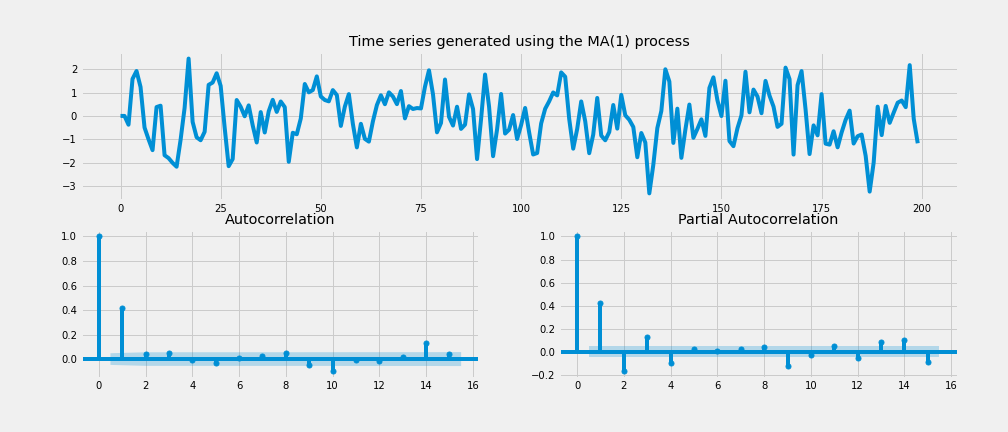
\includegraphics[width=1\textwidth, height=0.5\textwidth]{figures/chapter_03/ma_1_half.png}
  \label{fig:ma_1_half_example}} \\
  \subfloat[b][Time series generated using the MA(1) process with $\theta_1 = 2$.]{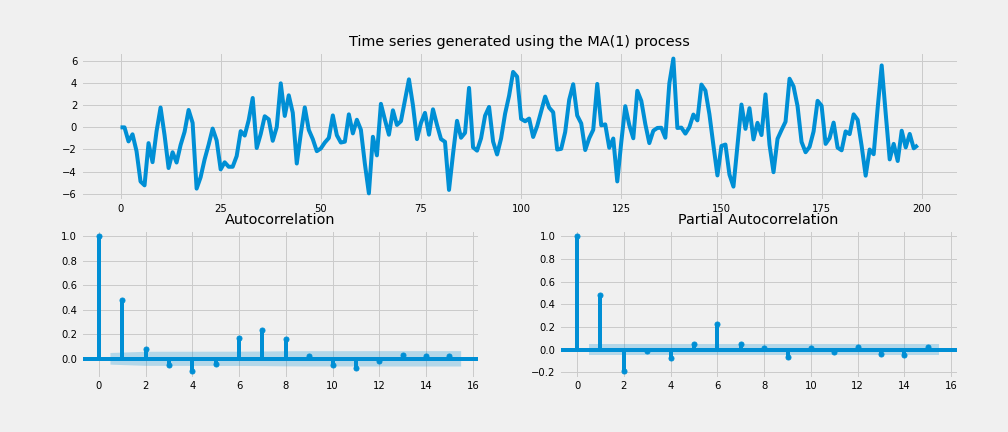
\includegraphics[width=1\textwidth, height=0.5\textwidth]{figures/chapter_03/ma_1_2.png} 
  \label{fig:ma_1_2_example}}
  \caption{Examples of the MA(1) process with identical value of ACF and PACF at lag 1.}
  \label{fig:ma_1_example}
\end{figure}

\subsubsection{Example of the MA(1) process}

Figure \ref{fig:ma_1_example} shows two examples of the MA(1) process with $\theta_1 = 0.5$ (Figure \ref{fig:ma_1_half_example}) and $\theta_1 = 2$ (Figure \ref{fig:ma_1_2_example}). It also demonstrates the related autocorrelation and partial autocorrelation functions. 

It is visible that the ACF and PACF drop after lag 1 ($q = 1$). Moreover, we are unable to guess the curtain value of $\theta_1$ parameter from the shape of these functions.

This find leads to the following property of the MA processes.

\subsubsection{Invertibility of the MA process}

According to Cryer et al. \cite{cryer2008time}, some MA($q$) processes can be reexpressed as an autoregression. Thus, if we consider MA(1) process (similar order as in previous section examples)
\begin{equation}
    Y_t = e_t + \theta_{1}e_{t-1},
\end{equation}
we can rewrite it as (with the similar form of $e_{t-1}$)
\begin{equation}
\begin{aligned}
e_t &= Y_t - \theta_{1}(Y_{t-1} - \theta_{1}e_{t-2})
&= Y_t - \theta_{1}Y_{t-1} + \theta_{1}^{2}e_{t-2}.
\end{aligned}
\end{equation}
If $|\theta_1| < 1$, we would not get exponential growth of $Y_t$ dependence on previous values and could continue infinitely
\begin{equation}
    e_t = Y_t - \theta_{1}Y_{t-1} - \theta_{1}^{2}Y_{t-2} - \ldots
\end{equation}
or 
\begin{equation}
    Y_t = e_t + \theta_{1}Y_{t-1} + \theta_{1}^{2}Y_{t-2} + \ldots
\end{equation}
It is now clear that the MA(1) model can be inverted into infinite-order autoregressive model if $|\theta_1| < 1$ and can be named \textbf{invertible}.

Before formulating the definition of the general MA($q$) model invertibility, we need to define its characteristic polynomial \cite{cryer2008time}.

\begin{definition}[\textbf{MA characteristic polynomial}]
\textit{Let us assume an MA process, $Y_t = \phi_{1}Y_{t-1} + \phi_{1}Y_{t-1} + \ldots + \phi_{p}Y_{t-p} + e_t$, then the \textbf{MA polynomial} is defined as \begin{equation}
    \theta(x) = 1 - \theta_{1}x - \theta_{2}x^2 - \ldots - \theta_{q}x^{q},
    \label{eq_ma_polynomial}
\end{equation} where $\theta_1, \ldots, \theta_p$ are the regression coefficients, and $x^1, \ldots, x^p$ are the complex numbers.
Therefore, the corresponding \textbf{MA characteristic equation} is \begin{equation}
    1 - \theta_{1}x^{1} - \ldots - \theta_{p}x^{p} = 0.
    \label{eq_ma_pol_eq}
\end{equation}}
\label{def_ma_char_polynomial}
\end{definition}

Now we can introduce the following definition.

\begin{definition}[\textbf{Invertibility of MA($q$) model} \cite{cryer2008time}]
\textit{Let us assume an MA process, $Y_t = \phi_{1}Y_{t-1} + \phi_{1}Y_{t-1} + \ldots + \phi_{p}Y_{t-p} + e_t$ and the model MA($q$) that describes this process. This model is \textbf{invertible}, if the are coefficients $\pi_j$ such that
\begin{equation}
    Y_t = \pi_{1}Y_{t-1} + \pi_{2}Y_{t-2} + \ldots + e_t,
\end{equation}
which is possible \textbf{if and only if} the roots of the corresponding characteristic equation $\theta(x) = 0$ \textbf{exceeded one in absolute value.}
\label{def_ma_invertibility}}
\end{definition}

Therefore, if we return back to the example in previous subsection, we may now notice that even if both processes have the same ACF, only one of them (with $\theta_1 = 0.5$) is invertible. 

To summarize this subsection, i would say that the \textbf{invertibility} of the MA process can be used to curtain estimation of its coefficients.

\subsection{Autoregressive Moving Average, ARMA model}

Sometimes, assuming that the process is only AR or only MA is not enough. In situations like this, we consider a mixed model named \textit{Autoregressive Moving Average} (denoted as ARMA($p, q$)) of orders $p$ and $q$. This leads to the following definition.

\begin{definition}[\textbf{Autoregressive Moving Average process of orders $p$ and $q$} \cite{shumway2011}]
\textit{Let us assume a stochastic process $Y = \left\{Y_{t}\;|\;t \in T\right\}$. This process can be named \textbf{the Autoregressive Moving Average of orders $p$ and $q$} if \begin{equation}
    Y_t = \phi_{1}Y_{t-1} + \ldots + \phi_{p}Y_{t-p} + e_t + \theta_{1}e_{t-1} + \ldots + \theta_{q}e_{t-q},
    \label{eq_arma_process}
\end{equation}
where the variables of the equation are 
\begin{itemize}
    \item $\phi_1, \ldots, \phi_p$ and $\theta_1, \ldots, \theta_q$ --- model parameters ($\phi_p \neq 0, \theta_q \neq 0$).
    \item $Y_{t-1}, \ldots, Y_{t-p}$ --- most recent $p$ past values.
    \item $e_{t}, \ldots, e_{t-q}$ --- the Gaussian white noise with zero mean and variance $\sigma_{e}^2$ at timestamp $t$ and $q$ more recent timestamps before $t$, unless otherwise stated.
\end{itemize}
If we talk about the ARMA process with nonzero mean value $\mu$, we need to replace $Y_t$ with $Y_t - \mu$ in Equation \ref{eq_arma_process}, \begin{equation}
\begin{aligned}
    Y_t - \mu &= \phi_{1}(Y_{t-1} - \mu) + \ldots + \phi_{p}(Y_{t-p} - \mu) + \\ &+ e_t + \theta_{1}e_{t-1} + \ldots + \theta_{q}e_{t-q},
\end{aligned}
\end{equation}
or write \begin{equation}
\begin{aligned}
    Y_t &= \phi_{0} + \phi_{1}Y_{t-1} + \ldots + \phi_{p}Y_{t-p} + e_t + \theta_{1}e_{t-1} + \ldots + \theta_{q}e_{t-q},
    \label{eq_arma_process_non_zero_mean}
\end{aligned}
\end{equation}
where $\phi_0 = \mu(1 -  \phi_0 -  \phi_1 - \ldots - \phi_p)$.}

\textit{The parameters $p$ and $q$ are usually called the autoregressive and the moving average orders, respectively. In addition, the process introduced in Equation \ref{eq_arma_process} can be described using the ARMA($p, q$) model if its AR part is \textbf{stationary} (Definition \ref{def_ar_stationarity}). Moreover, for the curtain estimation of the MA coefficients, we may use the MA process \textbf{invertiblity} (Definition \ref{def_ma_invertibility}).}
\label{def_arma_process}
\end{definition}

\begin{figure}[!ht]
\centering
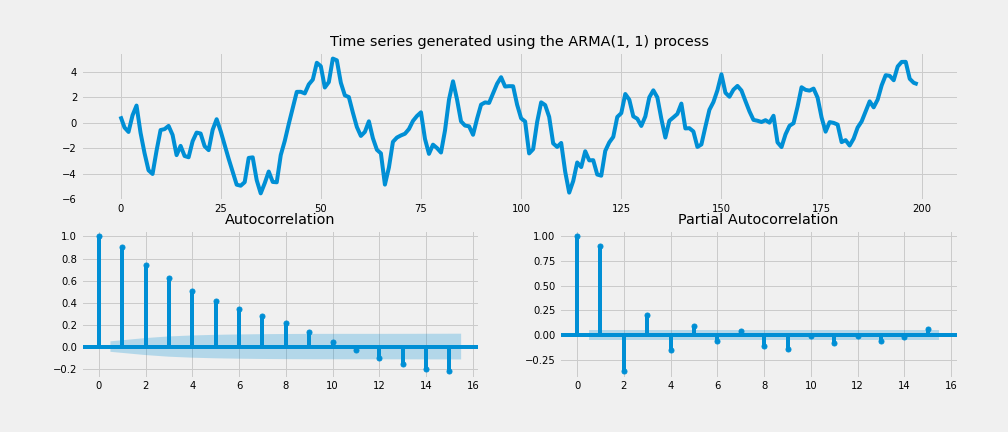
\includegraphics[width=1\textwidth, height=0.5\textwidth]{figures/chapter_03/arma_1_1.png}
\caption{The zero mean ARMA(1, 1) process example with its ACF and PACF: $\phi_1 = 0.8, \theta_0 = 0.5, Y_0 = 0.5$.}
\label{fig:arma_1_1_example}
\end{figure}

It is clear that if we assume $p = 0$, then the model will be a basic moving average of order $q$ or if we assume $q = 0$, then the model will be a basic autoregressive moving average of order $p$. 

Exploiting the fact that ARMA($p, q$) process is a mix of AR($p$) and MA($q$), we can rewrite Equation \ref{eq_arma_process} in a more compact form, using the autoregressive operator introduced in Equation \ref{eq_ar_operator} and the moving average operator introduced in Equation \ref{eq_ma_operator} as

\begin{equation}
    \phi(B)Y_t = \theta(B)e_t.
\end{equation}

\subsubsection{Example of ARMA(1, 1) process}

Figure \ref{fig:arma_1_1_example} demonstrates an example of
the time series generated with the ARMA(1, 1) process. The ACF and PACF indicate strong autocorrelation at lag 1. 

However, If we also take to account the example of the AR(1) process in Figure \ref{fig:ar_1_example}, we will notice that it is hard to guess the curtain order of the mixed ARMA model. The shapes of its ACF and PACF are similar to those related to the standard AR(1) process.  

\subsection{Integrated time series: Differencing \& ARIMA model}

All models introduced in the previous subsections required a (weakly) stationary process. However, a large number of real-life problems consist of nonstationary time series generated by nonstationary processes. For example, the random walk process (introduced in Definition \ref{def_random_walk}) has a constant mean but has no deterministic trend. It means that it can not be described using a model that assumes, for example, a stationary time series with an added time-varying mean $\mu$.

It is clear from the definition of random walk that it is a nonstationary AR(1) process given by
\begin{equation}
    Y_t = Y_{t-1} + e_t.
\end{equation}
However, by rewriting this process using the \textbf{first difference} defined as
\begin{equation}
    \nabla Y_t = Y_t - Y_{t-1},
\end{equation}
we will receive the following equation
\begin{equation}
    \nabla Y_t = e_t,
\end{equation}
which describes a stationary process. It is clear that this example can be easily extended to get not just the white noise.

In Cryer et al. \cite{cryer2008time} we can find an example, which assumes the process defined as \begin{equation}
    Y_t = M_t + X_t,
\label{eq_example_diff_ts}
\end{equation}
where $M_t$ is an almost constant (either deterministic or stochastic) series. It is possible to approximate the value of $M$ at timestamp $t$: \begin{equation}
    \hat{M_t} = \frac{1}{2}(Y_t + Y_{t-1}).
\end{equation} After this, we can get rid of $M_t$ in Equation \ref{eq_example_diff_ts} and receive \begin{equation}
    Y_t - \hat{M} = Y_t - \frac{1}{2}(Y_t - Y_{t-1}) = \frac{1}{2}(Y_t - Y_{t-1}) = \frac{1}{2}\nabla Y_t,
\end{equation}
which is a \textbf{constant multiple of the first difference at lag 1}.

This example assumes that $M$ in Equation \ref{eq_example_diff_ts} is stochastic and its changes are driven by the random walk process (along with $Y_t$), such that \begin{equation}
\begin{aligned}
    Y_t &= M_t + e_t, \\
    M_t &= M_{t-1} + \varepsilon_t,
\end{aligned}
\end{equation}
where $e_t$ and $\varepsilon_t$ are independent values generated by the white noise process. Then \begin{equation}
    \nabla Y_t = \nabla M_t + \nabla e_t = \varepsilon_t + e_t - e_{t-1},
\label{eq_example_diff_then_ma}
\end{equation}
which will have the autocorrelation function of an MA(1) process. According to Cryer et al. \cite{cryer2008time}, we can study $\nabla Y_t$ from Equation \ref{eq_example_diff_then_ma} as stationary.

It is also possible to formulate assumptions which will lead to a time series that will be stationary after the second difference, and so on. This motivates the following definition.

\begin{definition}[\textbf{Integrated Moving Average process ARIMA($p, d, q$)} \cite{cryer2008time}]
\textit{
Let us assume a stochastic process $Y = \left\{Y_{t}\;|\;t \in T\right\}$. This process can be described using \textbf{the Integrated Moving Average model} if the $d$th difference 
\begin{equation}
    W_t = \nabla^d Y_t
\end{equation}
is a \textbf{stationary ARMA process} introduced in Definition \ref{def_arma_process}. If $W_t$ can be described using ARMA model, we can say that $Y_t$ is an \textbf{ARIMA($p, d, q$) process}.
}
\end{definition} 
The most common values of $d$ that can occur in practice are 1 or 2. Therefore, we can introduce ARIMA process equation with $W_t = Y_t - Y_{t-1}$: \begin{equation}\begin{aligned}
W_t &= \phi_{1}W_{t-1} + \phi_{2}W_{t-2} + \ldots + \phi_{p}W_{t-p} \\ 
    &+ e_t + \theta_{1}e_{t-1} + \theta_{2}e_{t-2} + \ldots + \theta_{q}e_{t-q}.
\end{aligned}
\label{eq_arima_process}
\end{equation}
It is possible to rewrite this equation in terms of the original model, \begin{equation}
\begin{aligned}
Y_t - Y_{t-1} &= \phi_{1}(Y_{t-1} - Y{t-2}) + \phi_{2}(Y_{t-2} - Y{t-3}) \\
&+ \ldots + \phi_{p}(Y_{t-p} - Y_{t-p-1})\\
&+ e_t + \theta_{1}e_{t-1} +  e_t + \theta_{1}e_{t-1} + \ldots + \theta_{q}e_{t-q},
\end{aligned}
\end{equation}
or using \textbf{the difference equation form} of the model \cite{cryer2008time} as \begin{equation}
\begin{aligned}
Y_t &= (1 + \phi_{1})Y_{t-1} + (\phi_{2} - \phi_{1})Y_{t-2} + (\phi_{3} - \phi_{2})Y_{t-3}\\
&+ \ldots + (\phi_{p} - \phi_{p-1})Y_{t-p} - \phi_{p}Y_{t-p-1} \\
&+ e_t + \theta_{1}e_{t-1} +  e_t + \theta_{1}e_{t-1} + \ldots + \theta_{q}e_{t-q}.
\end{aligned}
\label{eq_diff_eq_form}
\end{equation}
In accordance with Equation \ref{eq_diff_eq_form} we now have ARMA($p+1, q$) process. However, the corresponding AR characteristic polynomial is \begin{equation}
\begin{aligned}
    1 &- (1 + \phi_{1})x - (\phi_{2} - \phi_{1})x^2 - (\phi_{3} - \phi_{2})Y_{t-3})x^3 \\
    &- \ldots - (\phi_{p} - \phi_{p-1})x^p `+ \phi_{p}x^{p+1}\\
    &= (1 - \phi_{1}x - \phi_{2}x^2 - \ldots - \phi_{p}x^p)(1 - x),
\end{aligned}
\end{equation}
which shows the root $x = 1$ that applies \textit{nonstationarity}. However, we obtain the remaining roots from the characteristic polynomial of the \textit{stationary process $\nabla Y_t$}. 

\begin{figure}[!ht]
\centering
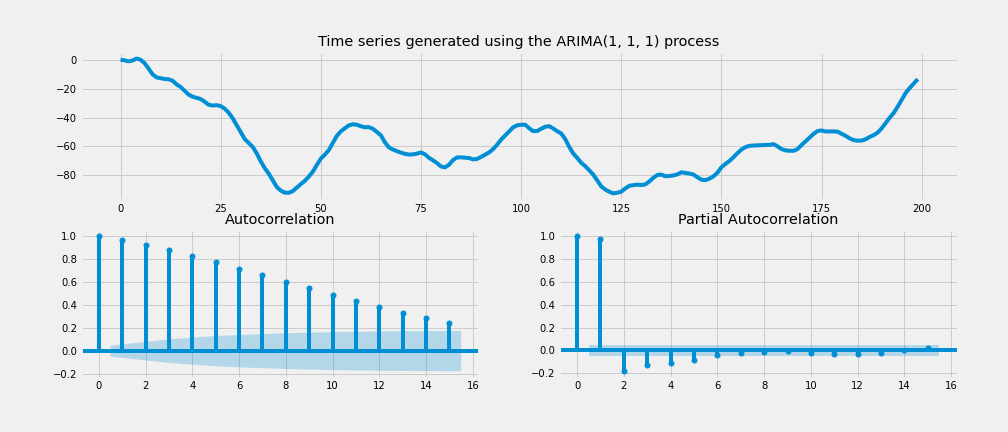
\includegraphics[width=1\textwidth, height=0.5\textwidth]{figures/chapter_03/arima_1_1_1.png}
\caption{The ARIMA(1, 1, 1) process example with its ACF and PACF: $\phi_1 = 0.8, \theta_0 = 0.5, Y_0 = 0.5$.}
\label{fig:arima_1_1_1_example}
\end{figure}

We can also formulate the ARIMA($p, d, q$) model more a more compact way using the autoregressive and moving average operators as \begin{equation}
    \phi(B)\nabla^{d}Y_t = \theta(B)e_t.
\end{equation} It is important to admit that if the process consists of only autoregressive terms, we denote the model as ARI($p, d$), or if it consists of only moving average terms, it is denoted as IMA($d, q$).

\subsubsection{Example of the ARIMA(1, 1, 1) process}

In Figure \ref{fig:arima_1_1_1_example} we can see the time series generated with ARIMA(1, 1, 1) process (obtained using cumulative sum of the example ARMA(1, 1) process). 

The ACF indicates that with lag increase, measure of the correlation decreases slowly. According to the PACF, there is a strong correlation  at lag 1 (does not hints the possible order of the AR part or of the MA part).

\subsection{Seasonality in ARIMA and ARMA processes, SARIMA model}

In the previous subsections, we have introduced ARMA and ARIMA models that cover a large group of real-life time series. However, these models can not handle situations where the analyst needs to deal with (multivariate) seasonality (Definition \ref{def_seasonal}). For example, we can consider a time series related to some seasonal business near the sea. During summer we will repetitively obtain a bigger amount of visitors then during other months (yearly seasonality). Or if we consider a COVID-19 related time series with information about the daily number of people infected (Figure \ref{fig:daily_inf}), we would see a weekly seasonality (from Monday to Wednesday, the number reaches a peak, by Friday it gradually decreases; a sharp decrease on weekends). 

These facts lead to the modification of the ARMA and ARIMA models named \textit{Seasonal Integrated Autoregressive Moving Average} (SARIMA).

First, we need to describe the mathematical principal behind the seasonality in ARIMA model. It assumes that the value of the observed variable $Y$ at timestamp $t$ depends not only on the most recent previous observations but on the observations obtained at timestamps $t-s, t-2s, \ldots$ (where $s$ is the duration of the season). In other words, $Y_t$ also depends on the same points of the seasonal cycle back in the history. 
If we consider the pure seasonality dependence of $Y_t$, ARMA($P, Q)_{s}$ model \cite{shumway2011} can be introduced as \begin{equation}
    \Phi_{P}(B^s)Y_t = \Theta_Q(B^s)e_t,
\end{equation}
where \begin{itemize}
    \item $\Phi_{P}(B^s)$ is the \textbf{seasonal autoregressive operator of order $P$} and $\Theta_Q(B^s)$ is the \textbf{seasonal moving average operator of order $Q$}.
    \item $s$ is the seasonal period.
\end{itemize} In general, we assume that $Y_t$ depends on a mix of seasonal and nonseasonal components. This follows a mixed ARMA($p, q$) $\times$ ($P, Q)_s$ formulated as \begin{equation}
    \Phi_{P}(B^s)\phi(B)Y_t = \Theta_Q(B^s)\theta(B)e_t.
\end{equation} Moreover, if we assume a nonstationary process and add a differencing, we will obtain the following definition.

\begin{definition}[\textbf{Seasonal Integrated Autoregressive Moving Average process ARIMA($p, d, q$) $\times$ ($P, D, Q)_s$}]
\textit{
Let us assume a stochastic process $Y = \left\{Y_{t}\;|\;t \in T\right\}$. This process can named as \textbf{Seasonal Integrated Autoregressive Moving Average} if it can be described using \textbf{Seasonal Integrated Autoregressive Moving Average model} \cite{shumway2011} defined as \begin{equation}
    \Phi_{P}(B^s)\phi(B)\nabla^{D}_{s}\nabla^{d}Y_t = \Theta_Q(B^s)\theta(B)e_t,
\end{equation}
where the elements of the equation are:
\begin{itemize}
    \item $\Phi_{P}(B^s)$ and $\Theta_Q(B^s)$ --- the seasonal autoregressive of operator of order $P$ and the seasonal moving average operator of order $Q$, respectively.
    \item $\phi(B)$ and $\theta(B)$ --- the ordinary autoregressive of operator and the moving average operator, respectively.
    \item $\nabla^{D}_{s}$ --- seasonal difference component at lag $s$.
    \item $\nabla^{d}$ --- ordinary difference component at lag 1. 
    \item $e_t$ --- the Gaussian white noise with zero mean and variance $\sigma^2$.
\end{itemize}
}
\label{def_sarima_model}
\end{definition} 
Definition \ref{def_sarima_model} is the most important within the introduced in this section, because almost all time series considered in the practical part of this thesis can be described using this model with suitable parameters.

\begin{figure}[!ht]
\centering    
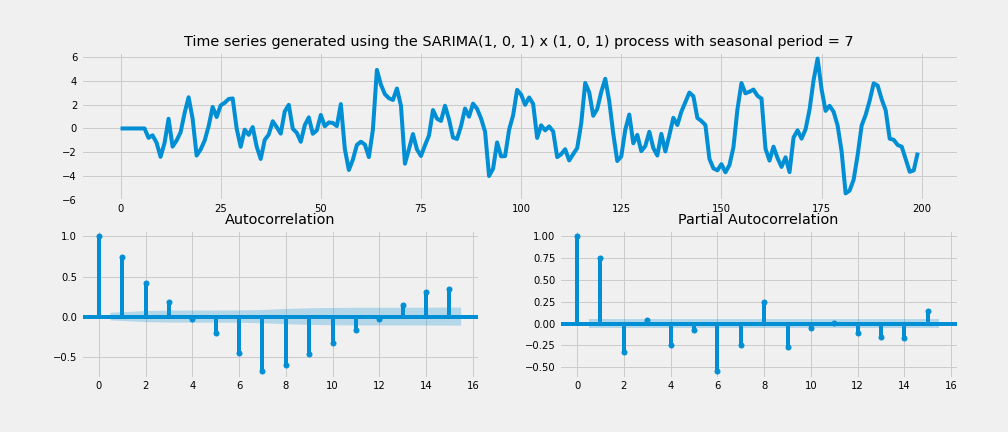
\includegraphics[width=1\textwidth,height=0.5\textwidth]{figures/chapter_03/sarima_example.png}    
\caption{The SARIMA(1, 0, 1) $\times$ (1, 0, 1$)_7$ process example with its ACF and PACF: $\phi_1 = 0.5,\Phi_1 = -0.4, \theta_0 = 0.4, \Theta_1 = -0.3$}    \label{fig:sarima_1_1_1_example}    
\end{figure}

\subsubsection{Example of the seasonal ARIMA time series}

Figure \ref{fig:sarima_1_1_1_example} demonstrates an example of the time series generated by the process denoted as SARIMA(1, 0, 1) $\times$ (1, 0, 1$)_7$. The ACF shows the most expressive autocorrelation at lags 1 and 7. We can also see that the pattern typical for AR processes takes its place not only after lag 1 but after lag 7. The PACF demonstrates correlation at lags 1 and 6.

According to this example, we can guess the possible seasonal period of the time series. However, estimation of the orders of the AR and MA parts is not a simple task.

\subsection{(S)ARIMA model building}

The (S)ARIMA model building consists of several steps. In Shumway et al. \cite{shumway2011} we found that it is possible to specify the following pipeline:
\begin{enumerate}
    \item plotting the data
    \item possible transforming the data
    \item identifying the order of the possible model
    \item parameter estimation
    \item diagnostics
    \item model choice
\end{enumerate}
The first step is common for every data analyst task. It is necessary to visualize the original data to create a list of future actions.

The second step means that sometimes we need to apply some data transformations. For example, if the variance of data increases over time, it will need some manipulations to stabilize the process (for example, \textbf{Box-Cox transformation} or some basic such as \textbf{logarithmic} \cite{osborne2010}). 

After a suitable data transformation, it is possible to estimate the order of the model. In other words, the estimation of general $p, d, q$ orders and seasonal $P, D, Q$. At the beginning of such a process, we need to estimate $d$ and $D$. We can perform differencing, after which we can look at the form of the obtained time series. The ACF and PACF could also be helpful. After $d$ and $D$, we can try to guess the order of the general and seasonal AR and MA components. The curtain estimation could not be possible at all, so we need to find at least approximately suitable values.

The following step implies model fitting. This can be done in a variety of ways. However, in this section we will introduce the \textit{maximum likelihood estimation} (MLE) method \cite{Hyndman2018}. In essence, we need to find parameters, which will maximize the probability of obtaining the original data with the given process. In case of (S)ARIMA it means the minimization of
\begin{equation}
    \sum_{t=1}^{T} \varepsilon_t = Y_t - \hat{Y_t},
\end{equation}
where T is the number of timestamps in historical data, $e_t$ is a residual (introduced, for example, in Equation \ref{eq_additive_model} and Equation \ref{eq_multiplicative_model}) at timestamp $t$, $Y_t$ is the value of the observed variable $Y$ at timestamp $t$, and $\hat{Y_t}$ is the estimated value of the $Y$ at timestamp $t$. It is also possible to coordinate the estimation process using the Akaike information criterion or the Bayesian information criterion.

Finally, we need to perform \textit{residual analysis}, that will be introduced in the practical part of this thesis. It will help us to measure the presence or absence of factors that influence our data but not described by our model (this step is also important for the Prophet model). 

After doing all this, we can start forecasting using our model.

\subsection{Forecasting using the (S)ARIMA model}

In essence, the forecasting with (S)ARIMA model can be shortly explained by a short sequence of actions \cite{Hyndman2018}. 

First, we need to rewrite the model equation for $Y_{T+h}$, where $T$ is the index of the most recent timestamp in the history and $h = 1, 2, \ldots$ is the index of the forecasted timestamp. While forecasting, we need to replace future observations with their forecasts, future errors with zero, and past errors with the corresponding model residuals. The confidential intervals for the forecast are computed according to the methods used in the curtain implementation of the (S)ARIMA model.

\subsection{Summary}

During the theoretical research, we discovered that the ARIMA and SARIMA models (with suitable parameters) can be used to predict the evolution of the COVID-19 pandemic processes. Various studies and researches introduced in at the beginning of this chapter confirm that.

This find, in conjunction with the properties of this kind of statistical models, led us to the fact that it would be a strong choice for modeling pandemic processes and comparation with the Facebook Prophet model.